% !Mode:: "TeX:UTF-8"
% !TEX root = ../main.tex
\chapter{绪论}

\section{研究课题的来源、背景及意义}

如今,圆柱绕流和多孔介质流动现象成为了人们研究的重要领域,尤其是近年来随着生物、医学及化学领域的快速发展,与之相关的多孔流动问题越来越多,等待着人们更进一步的研究。

在自然界和工程实践中,流体绕过钝体的流动是一种常见现象。船只在水面行驶,飞行器在空中航行,河水流过桥梁,海水绕过岛屿,风吹过高大的建筑物,这些都是钝体绕流的实例,它出现在世界的方方面面,与我们的生活息息相关。工程中如果未考虑到钝体绕流的某些特性,可能会发生严重后果,如图~\ref{fig: flow} a) 所示,1940 年 11 月,塔科马海峡吊桥崩塌,经证明这是由强风掠过时形成的卡门涡街引起共振而导致的事故,见示意图~\ref{fig: wind}。自然界的大气、海洋中出现的绕流现象如图~\ref{fig: flow} b) 所示,2017 年 1 月,冷空气在东北亚日本海上空凝结成了冷流云,冷流云南下掠过济州岛时在岛屿背后形成了漩涡结构。人们很早就对这种现象进行了思索和研究,随着流体力学基本理论的建立,人们对此类现象的认识也逐渐深刻起来。

\begin{figure}
	\setlength{\subfigcapskip}{-1bp}
	\centering
	\begin{minipage}{\textwidth}
		\centering
		\subfigure[塔科马海峡吊桥中部断裂]{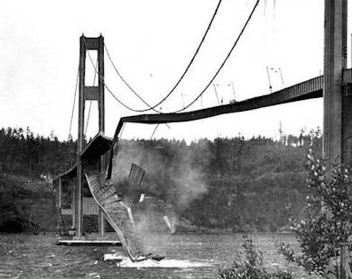
\includegraphics[width=.4\textwidth]{figs/bridge}}
		\hspace{2em}
		\subfigure[冷流云绕过济州岛]{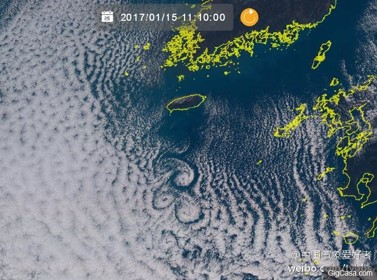
\includegraphics[width=.4\textwidth]{figs/cloud}}
	\end{minipage}
	\vskip 0.2em
	\wuhao 图片来源:a) Pinterest; b) http://www.wanhuajing.com/d688261
	\vspace{0.2em}
	\caption{钝体绕流现象举例}
	\label{fig: flow}
\end{figure}

\begin{figure}
	\centering
	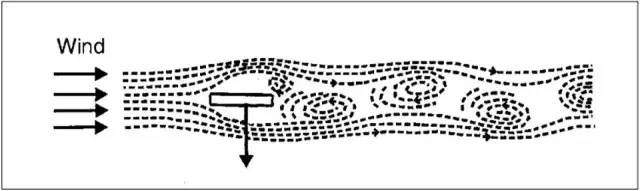
\includegraphics[width=.8\textwidth]{figs/wind}
	\vskip 0.2em
	\wuhao 图片来源:Bernard J. Feldman/The Physics Teacher.
	\vspace{0.2em}
	\caption{当稳定强风吹过桥梁(长方形)时产生漩涡,若风持续时间够长则改变桥梁的运动}
	\label{fig: wind}
\end{figure}

\section{国内外的研究进展及成果}

\subsection{圆柱绕流}

圆柱绕流是流体力学中的一个经典问题,按照雷诺数的划分,整个流动状态可以被划分为许多阶段 \cite{zdravkovich1997flow}。在远离圆柱的区域,流动可以按照势流理论处理。在靠近圆柱的区域,按流动特性可以将区域划分为四部分,参见图~\ref{fig: flow area}\cite{demartino2017aerodynamics}。这四个区域可分别称为缓流区、边界层区、边界区和尾迹区。当流体横掠平板时,从平板的前缘开始形成边界层,起初流态为层流状态,随着流体向下游的移动,层流逐渐转变为湍流状态。随着雷诺数的增加,层流转变为湍流的转变区也向上游移动。同样地,当流体流过圆柱时,在下游会出现流态的转变,随着雷诺数的增加,转变点也逐渐向上游移动,并且依次经过划分出来的几个区域,相应的流态称为尾迹区转捩(TrW)、剪切层转捩(TrSL)、边界层转捩(TrBL)。

\begin{figure}
	\centering
	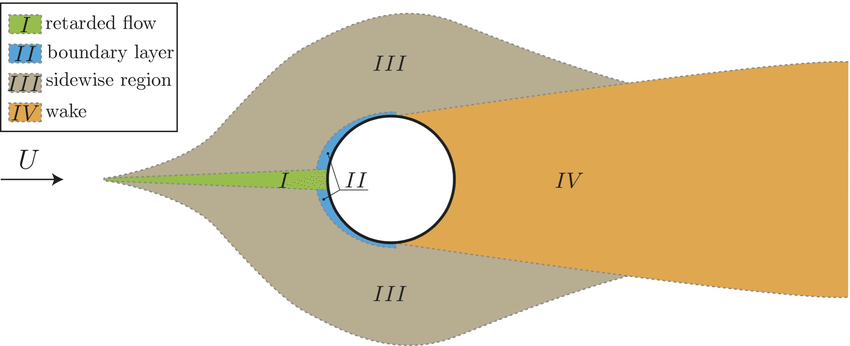
\includegraphics[width=.8\textwidth]{figs/Regions-of-disturbed-flow-around-a-perfect-circular-cylinder}
	\caption{流动区域的划分,图片摘自文献\inlinecite{demartino2017aerodynamics}}
	\label{fig: flow area}
\end{figure}

层流状态(L)。当 0 < $Re$ < 4--5 时,流体沿着圆柱的轮廓流动,圆柱左右的流线呈现出对称的特性,此时还没有出现流动分离。当 4--5 < $Re$ < 30--48 时,流体从圆柱表面分离,圆柱的背面开始出现封闭的附着涡,附着涡没有从圆柱表面脱落,此时尚处于稳定状态。当 30--48 < $Re$ < 180--200 时,圆柱背面的涡从圆柱表面脱落,并由近而远地向远处缓缓飘去。其中在 $Re$ > 30--48 时,尾迹区逐渐由稳态向非稳态过渡,尾迹末端的流线开始出现类似正弦曲线的摆动。随后,大约在 $Re$ > 45--65 时,剪切层卷起了一排排的波峰和波谷,接着出现了一列列的涡,即为涡街。

尾迹区转捩(TrW)。这一范围称为亚临界状态。当 180--200 < $Re$ < 220--250 时,首先在远离圆柱的尾迹区出现层流向湍流的转变(远尾迹转捩,TrW1),随着雷诺数的增大,转变点向上游移动。当 220--250 < $Re$ < 350--400 时,转变发生在接近圆柱的地方,称为近尾迹转捩(TrW2),最终,当涡一开始产生就已经处于湍流状态。TrW1和TrW2的一个重要现象是非稳态涡产生和脱落的层流模式逐渐被湍流模式所取代 \cite{zdravkovich1997flow}。

自由剪切层转捩(TrSL)。雷诺数处于这一范围的流动被称为亚临界状态。当 350--400 < $Re$ < 1k--2k 时,过渡波首先出现在近壁面剪切层,这一区域称为下亚临界区(TrSL1)。1k--2k < $Re$ < 20k--40k 时,过度涡出现在剪切层,在转变为湍流之前,过渡波沿着剪切层卷为分散的涡,之后则继续变成交替的涡,这一阶段为中亚临界区(TrSL2)。雷诺数范围为 20k--40k < $Re$ < 100k--200k 时是下亚临界区(TrSL3),此时近壁面处已全部转变为湍流状态,近壁面的自由剪切层突然转变为湍流,涡出现在圆柱的背面。

边界层转捩(TrBL)。这一状态也称为临界状态。100k--200k < $Re$ < 300k--340k 为前临界区(TrSL0),沿着分离线的剪切层开始转捩,阻力系数开始下降。300k--340k < $Re$ < 380k--400k 为单泡临界区(TrBL1),圆柱一侧的自由剪切层重附着形成分离泡。380k--400k < $Re$ < 0.5M--1M 为双泡临界区(TrBL2),圆柱两侧形成一对对称的分离泡。0.5M--1M < $Re$ < 3.4M--6M 为超临界区(TrBL3),此前出现的分离泡破碎,脱落涡丧失了周期性。3.5M--6M < $Re$ < unknown 为过临界区(TrBL4),此时边界层已完全转变为湍流,脱落涡周期性重现。这一阶段雷诺数的上界仍不为人所知。

完全湍流状态(T)。当雷诺数继续增大,整个流场变成了湍流状态。
%\cite{},非稳态层流 (?)
在圆柱绕流的几个阶段中,层流流动已经被较多地研究过,其中非稳态层流也有许多人研究。在非稳态区域,当雷诺数大于某个临界值 $Re_\text{osc}$ 时,原本处于稳态的层流就开始变得不稳定,圆柱尾部封闭的尾迹涡开始轻微振荡。临界雷诺数 $Re_\text{osc}$ 体现了尾迹的不稳定性,不同研究所揭示出的这一参数的具体数值有所不同 \cite{zdravkovich1997flow}。如果雷诺数小于临界值,尾迹也可以由外界激发而产生波动(例如弹性丝线的振动),随着外界干扰的平息,尾迹又会重新回归稳态。在实验研究中,人为施加的激励可以使临界雷诺数的大小降至 20 甚至 10,从而可以测出波动的频率,即 Strouhal 数。实验表明,由此得出的频率曲线可以和 $Re>Re_\text{osc}$ 时的频率曲线光滑衔接。

当雷诺数大于临界值时,近尾迹的不稳定将产生一个波浪形的痕迹,尾波开始卷起。Bénard 做了在糖水溶液中拖动圆柱的开创性实验,描述了尾迹处形成的漩涡。Phillips 通过实验发现,当 $40<Re<80$ 时,周期性的尾迹是二维结构,当 $80<Re<100$ 时,尾迹对扰动很敏感并可能变成三维的,当 $100<Re<160$ 时,尾迹就总是呈现三维结构了。也有其他一些实验的结果与此不太相同。

%许多努力都试图寻找为什么层流周期性尾迹会存在两种流动模式。

Strouhal 第一次利用金属丝和杆在空气中产生声音并测量了它的频率,提出了无量纲参数 $fD/V$, 后来被称为 Strouhal 数。他的研究发现,对细金属丝($400<Re<1k$)而言,$St=0.185$;对金属杆($1.8k<Re<5.4k$)而言,$St=0.195$。当 $40<Re<160$ 时,关系 $Re=\text{常数}$ 并不成立,此时,$St-Re$ 的关系是非线性的。Roshko \cite{Roshko1953} 得到的 $St-Re$ 关系为
\begin{equation}
	St = 0.212 (1-\frac{21.2}{Re})
\end{equation}
Roshko \cite{Roshko1953} 提出了一个新的无量纲数 $Ro=fD^2/\nu$ 从而使得 $Ro-Re$ 具有线性关系:
\begin{equation}
	Ro = 0.212 (Re - 21.2)
\end{equation}

Tritton 第一次使用了线性的 $Ro-Re$ 关系。在空气和水中,当 $Re>80$ 时,涡脱落的频率会有一个不连续的下降,并且发现,涡脱落频率的下降并不会对阻力产生影响。Tritton 注意到热金属丝产生的信号在不连续点以上和以下都很有规律,但处在不连续点附近的一个小范围内时,这些信号就变得不再那么规律。这种从一个模式到另一个模式的改变不一定发生在一个特定的 $Re$ 值,实际上,它可以发生在 $80<Re<105$ 的范围内。Tritton 认为,这种不连续是由封闭尾迹的突然消失和紧接着涡生成机制的改变引起的。这两种现象都会对阻力产生影响。Berger 发现,在 $Re=125$ 以上,$Ro$ 也有类似的不连续现象,并发现在 $125<Re<160$ 范围内存在两种亚稳态模式:一种是 Tritton 的高速模式,另一种低速模式被 Berger 称为“基础模式”,因为信号的幅值和相位都很有规律。这很可能是由圆柱的振动引起的。许多研究者都试图找到脱落的不连续点所对应的临界雷诺数 $Re_d$。Gaster 通过减小圆柱的长径比抑制了高速模式。Nishioka 和 Sato 将长径比减小到 $L/D=6$,不但抑制了原来存在的不连续性,而且将涡脱落时的临界雷诺数推移到了 $Re_\text{osc}=85$。Friehe 确信,脱落频率和 $Re_d$ 都严重依赖于 $L/D$。

Teissié-Solier 等人于 1937 年发现,一个固定直径的圆柱在一个测试段中产生了两个不同的频率。他们测量了沿着中心间隔的高频和沿着尾迹的低频。低频部分的范围是 $6D-8D$,并且在 $Re>214$ 时消失。Gerrard 测出 $Re=85$ 从尾端数 $7D$ 的距离时频率低了 16\%,证明了壁面涡街的存在。Gerich 和 Eckelmann 随后的研究确认了沿着圆柱展向的不同脱落频率的存在以及它们的范围。%都是什么?……

从波浪形尾迹到充分发展的交错涡街的演变影响着圆柱表面的压力分布。Thom 和 Homann 分别于 1928 年和 1936 年在水中和油中测量了层流状态下的压力分布。Williamson 和 Roshko 重复了测试并测量了在空气中的压差阻力 $C_{pb}$。在 $40<Re<170$ 范围内,$C_{pb}$ 从 $-0.5$ 变化到 $-0.9$。$L_f$ 的减小是和 $C_{pb}$ 的增大相关联的,因为涡已经在圆柱的附近形成了。Dimopoulos 和 Hanratty 通过使用电化学的方法测量了层流周期性流动状态下圆柱表面的阻力分布。当 $Re=60$ 时,$C_f$ 的最大值大约是 $60^\circ$;当 $Re=227$ 时,$C_f$ 的最大值大约是 $50^\circ$。随着 $Re$ 的增大,$C_{f\text{max}}$ 的值也在增大。$C_f=0$ 的点意味着分离现象的发生。对于 $Re=60$,分离发生的角度是 $\theta_s=115^\circ$;对于 $Re=227$,分离角度则渐渐变成了 $\theta_s=105^\circ$。在 $60<Re<150$ 范围内 $\theta_s$ 的微小变化标志着圆柱背面近尾迹尺寸的减小。Dimopoulos 和 Hanratty 证明,在圆柱背面放置一个平板不会改变 $\theta_s$ 的大小。作用在圆柱上的阻力包括摩擦阻力和压差阻力,分别由摩擦力和压力差产生。阻力 $C_D$ 在 $40<Re<160$ 范围内的变化是 $1.3<C_D<1.7$,小于 $5<Re<40$ 范围内的变化 $1.7<C_D<5$。波动的升力。Tanida 等人通过在一个油槽里拖动圆柱测量了周期性层流状态 $L3$ 下的波动升力。$Re=100$ 时 最大值 $C_L^\prime=0.08$,这说明圆柱附近的压力波动是非常微弱的。Roshko 测量了 $Re=150$ 和 500 时尾迹的波动动能。$Re=150$ 时大部分的动能都在脱落频率 $\overline{{u_1^\prime}^2}$ 附近,并在 $y/D=1.0$ 的位置达到了最大值。对于 $y/D < 1$,第一谐振出现在 $\overline{{u_2^\prime}^2}$ 并在尾迹轴线 $y/D=0$ 的位置达到最大值。对于 $Re=500$ 的湍流尾迹,最大能量出现在 $y/D=0.5$ 的位置,并且第一谐振和随机波动 $\overline{{u_r^\prime}^2}$ 相比几乎总是可以忽略不计。

\subsection{多孔介质内部的流动}

流体通过多孔介质的流动是地下水水文学、石油工程、土壤学及化学工程等领域的常见现象 \cite{Bear2013}。地下水水文学和采油工程中常常研究的含水层和储油层是多孔介质的两个典型例子(参见图~\ref{fig: Aquifers and oil reservoirs})。含水层又被称为地下水盆地,是一种含有水的地层或岩层,在一般的野外条件下允许大量的水在其中流动。储油层(和储气层)是一种多孔地层,它的多孔结构内除了含水,还含有至少一种呈现液相或气相的碳氢化合物(石油或天然气)。除地下水中的含水层和石油工程中的储油层外,土壤、多孔岩石、陶瓷、过滤纸和沙过滤器乃至广泛分布于中国华南地区的岩溶地貌(喀斯特地貌)都是多孔介质的实例。此外,流化床、生物过滤器、森林中的降雨、生物工程中的微载体和支架以及多孔换热器也都是多孔介质流动的重要研究领域。

\begin{figure}
	\centering
	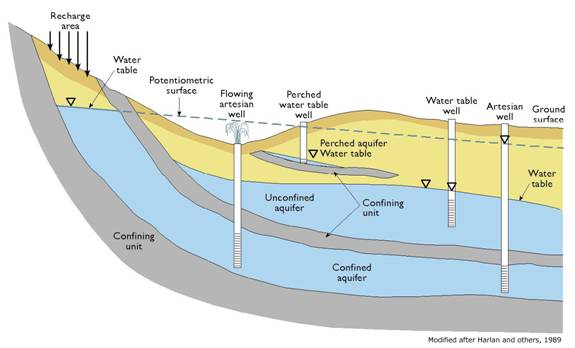
\includegraphics[height=.2\textheight]{figs/Aquifers}
	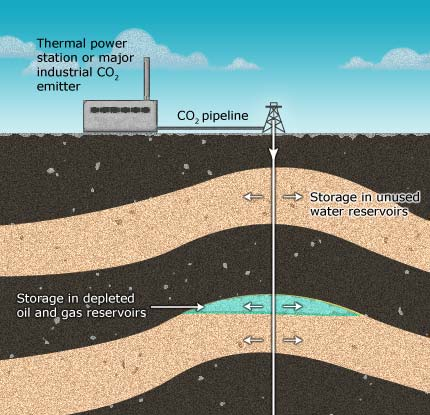
\includegraphics[height=.2\textheight]{figs/Oil-reservoirs}
	\vskip 0.2em
	\wuhao 图片来源: Colorado Geological Society; Alan Sherwood and Jock Phillips, 'Coal and coal mining - The future of coal', Te Ara - the Encyclopedia of New Zealand
	\vspace{0.2em}
	\caption{含水层和储油层}
	\label{fig: Aquifers and oil reservoirs}
\end{figure}

多孔介质可以简单描述为“含有孔洞的固体”,从流体流动的角度来说,它是多相物质占据的空间,且有一相需为固体;固相分布在整个多孔区域;一部分孔隙必须互相连通,使得气液相的流体可以在其中流动 \cite{Bear2013}。

虽然经典力学可以描述若干分子组成的分子体系的运动,但由于流体中包含了大量的分子,从分子水平上对每一个流体粒子进行描述显得徒劳无力。事实上,仅仅处理三个分子的运动问题也是十分困难的。我们难以从分子水平去处理流体的运动,转而利用统计的方法解决问题,求出由许多个分子组成的系统的整体运动信息。这样由若干分子组成的一个系统便称为“流体质点”,流体被看作是由无数流体质点所组成的连续介质。这样的流体连续介质水平被称为“微观水平”。在处理问题时,组成流体的分子结构被忽略,描述问题的角度从分子水平迈向了微观水平。

%在流体质点和连续介质假设的基础上可以定义流体的密度

在多孔介质中,被视为连续介质的流体在孔隙中流动,按照前述假设,我们可以确定每一点上流体的物理和运动性质。然而,由于多孔介质孔隙内部复杂的几何边界,我们无法用数学方法准确地描述固体的几何形状,也无法确定相应的边界条件。所以,流体连续介质的假设无法解决多孔介质内的流动问题。为了克服这一困难,应当转向更粗的平均水平,即转向宏观水平——也是更高水平的连续介质方法。

类比于流体质点的概念,多孔介质中可以定义表征性体积单元(representative elementary volume, REV)的概念。表征体元的尺寸应该小于整个流动区域,同时又要包含足够多的孔隙。类比流体密度的定义,孔隙率定义为多孔骨架中空隙体积占总体积的比重,并且是空间位置的连续函数。通过引入孔隙率和表征体元,实际的多孔介质被视为连续介质,描述问题的尺度从微观水平转到了宏观水平。在这个假设的基础上,我们可以用连续函数来描述多孔介质内的流动,并由此建立起相应的质量方程和动量方程。

%流体的连续介质假设将对流体的描述从分子尺度转移到流体质点尺度(微观水平)。类比对流体的描述,我们引入多孔介质的连续介质假设,这样就将描述水平进一步转到表征体积单元(REV)的尺度上(宏观水平)。

在描述多孔介质流动方面,Darcy 定律和 Brinkman 方程是两个主要的模型。heikholeslami\cite{Sheikholeslami2017} 在多孔圆柱微纳流动的研究中就采用了达西模型。这两个模型都不含时间的导数项和非线性的对流性。Wang L 等人 \cite{Wang2015} 通过采用体积平均法,从具有孔隙尺度的宏观方程中严格推导出了包含时间导数项和非线性对流项的控制方程,对此方程应用蠕动流条件可以推导Darcy定律和Brinkman方程。该方程对内部项平均速度和相平均速度均满足伽利略不变性,具有现实的物理意义。为了验证得到的结果,该文献采LB方法求解了多孔圆柱沿槽道中心线运动的问题,并且模拟了多孔通道中的Poiseuille流动,与有限差分的结果相一致。在此基础上建议使用内部相平均速度而放弃使用通常用于多孔粒子系统的相平均速度。%?

\subsection{绕过及穿过多孔钝体的流动}

由于在自然界和工程中的普遍性,钝体绕流现象一直是人们研究的重要内容。

到目前为止,人们针对钝体绕流现象已经做出了大量研究,得到了许多有意义的结果。Joseph 和Tao \cite{joseph1964effect} 采用 Darcy 定律与 Stokes 渐进方程研究了低雷诺数下流体绕过多孔球体的粘性不可压缩流动,得到了速度场、压力场和阻力系数的解析解。Neale 等 \cite{neale1973creeping} 探究了 Brinkman 项对多孔球体绕流的影响,结果发现,在低雷诺数条件下,多孔圆柱受到的阻力要低于相同条件下的实心圆柱。Masliyah 和 Polikar \cite{masliyah1980terminal} 通过实验验证了 Neale 等人的结果。接着,Masliyah 和 Polikar \cite{masliyah1980terminal} 进一步发现,在高雷诺数条件下(7 < $Re$ < 120),多孔球体受到的阻力可能会高于相同条件下的实心球体。Nandakumar 和 Masliyah \cite{nandakumar1982laminar} 通过研究发现,Masliyah 和 Polikar 预测的阻力数值比他们的数值模拟结果高出大约 10\%。

Hsu 等人 \cite{hsu2004re} 采用 Brinkman 模型研究了低雷诺数下流体绕过多孔球壳的流动。Bhattacharyya 和 Raja Sekhar \cite{bhattacharyya2004viscous} 研究的多孔球体模型有一个不允许流体通过的中心,他们研究了穿过这个多孔球体模型的 Stokes 流动,其中多孔介质内的流动采用了 Brinkman 模型,多孔介质和纯流体之间的界面上采用了应力阶跃条件 \cite{ochoa1995momentum1,ochoa1995momentum2}。结果发现,应力阶跃系数对作用在该球体上的阻力和转矩都有着显著的影响。Rashidi\cite{Rashidi2015} 探究了多孔介质圆柱的应力阶跃条件。%?

Jue \cite{jue2004numerical} 探究了当 $Re$ = 100, 200 和 250 时多孔圆柱绕流中圆柱背面涡的脱落情况。他的研究基于有限单元法,采用了通用的非 Darcy 多孔介质模型,并在处理纯流体和多孔介质界面处的流动特性时使用了调和平均数。研究发现,除雷诺数外,达西数对流动也有着显著的影响,但孔隙率的影响却无足轻重。Chen 等人 \cite{chen2008numerical} 研究了应力阶跃条件对多孔圆柱绕流的影响,结果显示,当达西数增大时,涡脱落现象发生时所对应的雷诺数也会随之增大。同时,界面应力阶跃参数对多孔圆柱绕流的稳定性有着重要影响,其中第一参数有明显的影响而第二参数影响很小。

Noymer 等人 \cite{noymer1998drag} 使用商业软件 PHOENICS 研究了圆柱绕流现象,Darcy 方程和 Navier-Stokes 方程分别用来描述多孔区和纯流体区的流动,在两种流动的界面上,压力和质量流量匹配在一起。结果显示,当 $Re$ = 100 和 1000 时,作用在多孔圆柱上的阻力要比无渗流的实心圆柱高得多。这一结论也被他们的风洞试验所证实。Bhattacharyya 等人 \cite{bhattacharyya2006fluid} 通过数值分析的方式研究了绕过及穿过多孔圆柱的稳定流动,多孔区域的流动采用了包含 Brinkman 项、Forcheimmer 项和非线性对流项的通用模型。结论显示,阻力系数、尾迹长度和流动分离的角度都会随着达西数的增大而减小。当达西数减小时,再循环尾迹产生时对应的临界雷诺数也会单调减小,最终减小到一个渐进值,即为绕实心圆柱流动产生涡时所对应的雷诺数。

Fransson 等人 \cite{fransson2004flow} 研究了连续抽气和吸气时的圆柱绕流情况,研究的雷诺数范围为 $10^4$ 量级,即处于亚临界区。研究发现即使中等程度的吸气或吹起对流场都有着明显的影响。吸气可以延迟流动分离的发生,缩小尾迹的宽度,减小阻力,吹气具有相反的效果。

Yu 等人 \cite{Yu2011} 研究了绕过及穿过多孔圆柱流动的稳定状态,分析了雷诺数和达西数对流动的影响。结果发现圆柱背面的循环尾迹或穿入圆柱之内,或和圆柱相分离。多孔圆柱的尾迹从内部或下游开始发展,而不会像实心圆柱那样从表面开始。有限雷诺数下尾迹的形态是涡积累的结果,而非逆压梯度下的边界层分离所致。尾迹出现的临界雷诺数是达西数的函数;穿透深度是雷诺数和达西数的函数,类似地,文献 \inlinecite{Yu2010,Yu2012} 研究了多孔方柱和多孔球体的情形,也有类似的现象发生。

王亚玲 \cite{王亚玲2001圆柱绕流的三维数值模拟} 等人对圆柱绕流进行了三维数值模拟,采用有限体积法模拟了亚临界区内的绕流流动,计算结果表明,高雷诺数时圆柱周围的流动具有明显的三维特性,且沿柱长方向不同断面的升力和阻力系数并不相同,三维模拟的升力和阻力系数均小于二维模拟。而何鸿涛 \cite{何鸿涛2009圆柱绕流及其控制的数值模拟研究} 通过数值模拟的方法来研究圆柱绕流的基本特性,探究了三种控制方法对于圆柱绕流尾部涡脱落的控制效果。Amirul Hakam\cite{Hakam2018} 则研究了两个被动控制的圆柱绕流问题。

\subsection{存在的不足和有待深入研究的问题}

起初人们对这一问题的研究主要采用理论分析和解析计算的方法,随着计算机的发展,数值计算技术得到了迅速提高,与之相关的理论也层出不穷,极大地丰富了研究的手段。之后人们便主要利用数值模拟来研究此类问题了。同时也和实验相配合,验证结果的可信度,更深刻地理解其中的原理。另一方面,对流动基本原理的探讨也一直在进行中,包括对基本控制方程的改进和新的解释。

针对多孔圆柱绕流或与之相似的问题,人们通常研究的是低雷诺数绕钝体的流动,相应的钝体主要是几何形状简单的物体,例如球体、圆柱或是球壳、环形。一开始采用的模型主要是 Darcy 定律和 Brinkman 模型。后来,随着对流动控制方程认识的深入,更多的物理含义被发掘出来,于是,包含有 Brinkman 项、Forcheimmer 项和非线性对流项的通用模型被越来越多的人所采用。应力阶跃条件被用在对纯流体区域和多孔介质区域界面条件的处理上,但有研究指出应力阶跃条件对作用在球体上的阻力有着明显的影响。在实际的研究中,人们发现,相比于普通的绕流问题,绕流物体内部多孔介质的存在对流动有着重要的影响,主要是达西数和孔隙率的影响。当达西数增大时,涡脱落现象发生时所对应的雷诺数也会随之增大。而更有研究指出阻力系数、尾迹长度和流动分离的角度都会随着达西数的增大而减小。现有研究表明,在稳态流动时,多孔圆柱背面的尾迹回流区和普通圆柱有所不同。普通圆柱的尾迹区附着在圆柱表面,而多孔圆柱的回流区并没有附着在表面,而是和圆柱分离了一段距离,或者穿入了圆柱内部,甚至在雷诺数增加时还会消失,这些现象指示出稳态条件下多孔介质流动不同于普通圆柱的诸多特性。因此很有必要研究非稳态时,多孔介质和普通圆柱绕流的不同点。即流态发展到非稳态时多孔介质的存在又会对流动产生怎样的影响,以及多孔参数是如何对流动状态发生具体影响的,仍是需要进一步研究的问题。

\section{流体力学中的计算方法概述}

对于简单的流动问题,通过求解流体力学方程可以得到解析解,已知的解析解可以加深对流动机理的理解,但却很难直接用于工程分析和设计中。根据实际问题对方程进行简化并使用量纲分析来求解问题是一种可行的方法,主要适用于所研究的系统仅有一两个无量纲参数的情形。如果无量纲化的纳维尔-斯托克斯方程仅以雷诺数为独立参数,就常常使用这种方法。如果几何体的形状是固定不变的,我们可以通过相似模型实验得到想要的结果。时至今日,这种方法在实际工程设计中依然很有价值。问题在于,许多流动都需要若干个无量纲参数,可能无法建立起与实际流动相似的实验条件。例如,在飞机机翼的绕流中,为了利用更小的模型达到相同的雷诺数,就必须提高空气的流速,这可能会导致马赫数过高,为了避免这样的问题就要寻找合适的流体。在船只绕流问题中,同时满足雷诺数和弗劳德数也是几乎不可能的。与此同时,有的实验可能需要很高的成本。

随着电子计算机的诞生,计算的方法成为可能;随着计算机性能的提升和成本的下降,计算的手段也更加简易而高效。用计算机求解流体力学方程变得越来越重要,同时更多的人员使用这一方法研究流动现象,从而形成了计算流体力学这一研究领域。流动现象是用偏微分方程描述的,为了得到方程的数值解,使用离散方法将微分方程近似为代数方程然后求解,解的精度则取决于所使用的离散方法。

一个完整的数值方法应该从以下几个方面进行考虑。

(1)数学模型。包括偏微分方程和边界条件的建立。针对要解决的具体问题,选择合适的控制方程,这样的模型可能是对原始守恒方程作出一定的简化得到的。一种求解方法是针对一类特定的问题而提出来的,试图寻找可以求解所有流动问题的通用方法是不现实的;与此同时,适用性广的方法通常针对性较差,即在求解具体问题上不是最优的。

(2)离散方法。选择合适的离散方法对时间和空间进行离散,用得到的代数方程代替原来的微分方程。几种主要的方法是有限差分法(finite difference, FD)、有限体积法(finite volume, FV)和有限元法(finite element, FE)。谱方法(spectral scheme)、边界元法(boundary element)和元胞自动机(cellular automata)等其他方法适用于一些特殊的问题。

(3)坐标系和基向量的选取。流体力学的控制方程在不同的坐标系下具有不同的书写形式,例如直角坐标系、柱坐标系或球坐标系,正交或非正交坐标系下的表达方式也不相同。针对具体的流动选择合适的坐标系,这可能影响到离散方法和网格类型的选择。基向量的选择决定了向量和张量的定义,例如固定或可变、协变或逆变。速度向量和应力张量根据各坐标轴分解为各自的分量。

(4)网格划分。将问题所在的几何区域离散化处理,所有的变量就定义在这些离散后的位置上,最终目的是得到这些位置上各个变量的值。经过离散化处理,原先的求解区域被划分为大量的小区域。划分后的每个小区域——或称为网格——主要有以下几种形式。

\begin{enumerate}
	\item 结构化网格(structured grid)。
	\item 分块结构化网格(block-structured grid)。
	\item 非结构化网格(unstructured grid)。
\end{enumerate}

(5)有限近似。在离散化过程中需要选择近似的程度。有限差分方法中要选择网格点处导数的近似,有限体积方法中要选择面积分和体积分的近似,有限元方法中则要选择形状函数和权重函数。近似方法的选择影响到计算的精度,也影响到求解的困难程度、程序编写调试的难度以及程序运行的速度。最终需要在简单易行、精度和计算效率之间取得平衡。

(6)求解方法。离散之后的方程通常是一个庞大的非线性代数方程组。对于非稳态流动,通常像常微分方程的初值问题那样来求解。每经过一个时间步长都去求解一个椭圆形问题。稳定流动问题通常采用伪时间推进(pseudo-time marching)或一种等效迭代方法(equivalent iteration scheme)。由于方程是非线性的,所以要用迭代的方法求解。这些方法对方程进行线性化,得到的线性方程组几乎总是可以用迭代的技术进行求解。求解方法的选择取决于网格的类型和每一个线性方程中节点的数目。%等效迭代方法(equivalent iteration scheme)?

(7)收敛标准。对于迭代方法,要设置一个收敛的标准。通常情况下有两种迭代的级别:求解线性方程过程中的内部迭代和处理方程组之间的耦合及非线性关系过程中的外部迭代。无论是从精度还是效率的角度,迭代过程的终止条件都十分重要。

数值解法应当具有某些性质,大多数情况下不可能分析出完整的解方法,如果方法中的某一个环节不满足解的性质,那整个方法也不满足。以下是一些重要的性质。

(1)一致性。当网格间距趋向于零时,离散化应当变得精确。离散方程和真实方程之间的差距称为截断误差(truncation error),通常用泰勒级数在某个节点上展开的值与真实值的差来表示。当网格尺寸 $\Delta t \to 0$ 和/或 $\Delta x_i \to 0$ 时,具有一致性的方法应当使得截断误差为零。截断误差通常和网格尺寸 $\Delta x_i$ 和/或时间步长 $\Delta t$ 成正比,如果截断误差的主要项正比于 $(\Delta x_i)^n$ 或 $(\Delta t)^n$,则称为 $n$ 阶近似($n>0$)。%有些离散方法使截断误差成为 $\Delta x_i$ 和 $\Delta t$ 之比的函数,一致性的要求变成了:

即使解方法具有一致性,也不意味着离散方程组的解在小步长的极限下成为微分方程的解,因为解还需要具有稳定性。

(2)稳定性。解的稳定性要求它在求解过程中不会放大误差。对时间问题,稳定性保证了当实际解有边界时数值解也有边界。对迭代方法而言,稳定解意味着不会发散。稳定解不容易判断,尤其是当存在边界条件和非线性的时候。因此,常常在具有常系数、不含边界条件的线性问题时去验证稳定性。经验表明,用这种方式得到的结果通常可以用于更复杂的情况,除了部分例外。广泛采用的研究稳定性的方法是冯纽曼法(von Neumann's method)。

(3)收敛性。随着网格尺寸趋于零,离散方程的解趋于实际微分方程的解的时候,该方法具有收敛性。对于线性初值问题,Lax 等价理论(Lax equivalence theorem)\cite{Richtmyer1967}指出,给定一个合适的线性初值问题和有限差分近似,并且满足一致性条件,那么稳定性就成为收敛性的充要条件。对于受边界条件影响的非线性问题,稳定性和收敛性都难以验证。因此,收敛性通常使用数值实验来检验,例如,用一系列连续变化密度的网格重复计算,如果方法是稳定的并且离散过程中近似方法也都保持一致,最终的解就会收敛于一个网格无关的解。

(4)守恒性。求解的方程满足守恒率,相应的数值方法也同样应该满足。在稳定状态且不存在源和汇的情况下,离开一个控制体的守恒量等于进入这个控制体的量。如果对方程的守恒形式使用有限体积法,那么每一个小的控制体和整个求解区域都要满足守恒率。源和汇的处理应该是一致的,以使得整个区域内源和汇的代数和等于守恒量通过边界的净流率。守恒性是解方法的一个重要性质,因为它为解的误差强加了一个限制。如果质量守恒、动量守恒和能量守恒得不到保证,就会人为产生源和汇,改变局部和整体的平衡。

(5)有界性。数值解应该具有一定的边界,有的物理量不能取负值(例如密度、动能),有的量必须介于 0\% 和 100\% 之间(例如浓度);不存在源和汇时,一些方程要求物理量的最大最小值应在区域的边界上取得。数值解法应该考虑这些条件。有界性难以得到保证。仅有一阶格式可以保证这个性质,所有的高阶格式都会产生超出边界的解,但是这仅会在网格过于稀疏时发生。

(6)可实现性。过于复杂而无法直接处理的模型应该保证可以得到物理上真实的解。这并不是一个数值自身的问题,而是非现实的模型可能产生出非物理的解,或者造成数值方法的发散。

(7)准确性。数值解均为近似解,除了求解算法的误差、程序或边界条件的误差外,通常还包含三种误差:模型误差、离散误差和迭代误差。模型误差为实际流动和数学模型真实解之间的差距;离散误差为守恒方程真实解和离散之后得到的代数方程组真实解之间的差值;迭代误差为求解代数方程组时迭代得到的解和真实解之间的误差。有时,不同的误差可能相互抵消,因为如此,粗糙网格的误差可能比细密网格的误差更小。

通常使用的离散方法有有限差分、有限体积、有限单元法几种。

(1)有限差分法。有限差分是最早出现的求解偏微分方程的数值方法,被认为由欧拉于 18 世纪提出。求解开始于微分形式的守恒方程,求解区域划分为排列在一起的网格。在每一个网格点上,用函数在该节点的值代替该节点上的偏导数,微分方程得到近似。每个节点都将得到一个代数方程,该节点和邻近节点上的变量都作为未知变量而存在。原则上,有限差分法可以用于任何网格类型,但在实际中,它常被用于结构化网格。通常用泰勒级数展开或多项式拟合的方法得到变量的一阶和二阶导数,必要时,还可以用这些方法得到网格节点之外的其他节点上的变量值。对于结构化网格,有限差分法简单而有效,易于获得高阶格式,它的缺点在于守恒性不易实施,而且不适用于复杂的流动情形。

(2)有限体积法。有限体积法从积分形式的守恒方程开始,求解区域被划分为紧邻着的有限数量的控制体,在每一个控制体上应用守恒方程。每个控制体中心节点上的值待求,用插值的方法得到控制体每个面上的值(用中心节点的值表示),用合适的积分公式表示面积分和体积分,我们可以得到每个控制体上的代数方程,临近节点上的变量也出现在这个方程中。有限体积法适用于任何类型的网格,因此也适用于复杂的几何区域。网格仅定义了几何区域的边界,并且不需要和坐标系联系起来。只要具有同一边界的控制体具有相同的面积分,该方法就满足守恒性。有限体积法易于理解和编程实现,缺点在于,与有限差分相比,二阶以上的格式在三维情形中难以实现。

(3)有限单元法。有限单元法在许多方面都和有限体积法相似。求解区域被划分为一系列离散的控制体或有限单元,这些控制体一般是非结构的,二维情形下通常是三角形,三维情形下则是四面体或六面体。当在整个区域上积分时,方程前要乘以权重因子。在简单的有限元法中,解通过线性形状因子来近似,每个单元都确保解在单元边界上的连续性,这样的一个因子可以根据它在单元角点上的值来构建。权重因子也是同样的形式。然后,近似被代入守恒率的加权积分,通过令积分对每个节点值的导数为零,得到待求解的方程。最终得到非线性代数方程组。%?

本节内容主要阐述了流体力学中的计算方法。在实际问题中,有时解析和实验的方法无能为力,这时数值方法起到了重要作用,计算机的发展促进了数值计算的发展。数值方法应该包括多个组成部分,例如确定数学模型,选择恰当的离散方法,选取简易方便的坐标系和基向量,合理划分网格,兼顾计算精度和计算效率,选取求解方法,确定计算的收敛条件,等等。同时数值解法需要满足一定的性质,例如一致性、稳定性、收敛性、守恒性、有界性、可实现性和准确性等。常用的几种数值求解方法有限差分法、有限体积和有限单元法,各有一定的优缺点,适用于不同的场合。

\section{本文的主要研究内容}

%本课题的研究内容主要是

多孔圆柱流动中流动状态随雷诺数的变化和非多孔圆柱是相似的,当雷诺数不大时,垂直于圆柱轴线任一截面上的流态是相同的,此时的流动是二维问题。雷诺数较小时流动处于稳态,随着雷诺数的增大,圆柱的背面会出现漩涡。雷诺数继续增大,流态也渐渐变成非稳态,圆柱背面会出现两列对称的涡街,速度等流动参数也以一定的规律变化着。

对多孔圆柱绕流的研究通常关注稳定状态的流动,当雷诺数增大时,流动将变得不稳定,逐渐进入非稳定状态。对多孔圆柱绕流非稳态特性的研究就构成了本课题的主要内容。进一步地,课题的研究内容可以分为以下两个方面。

(1)层流非稳态情况下多孔圆柱绕流的数值模拟。

首先明确描述研究区域内流体流动的控制方程。由于控制方程是复杂的非线性偏微分方程,无法得到解析解,所以接下来要对方程进行离散化处理,利用计算流体力学的理论,采用合适的离散格式,运用数值求解技术来求解对应的方程,从而解决方程所描述的物理问题。最终得到所研究的流场内各个点上的数据,例如速度、涡量、压力等,以及不同条件下圆柱所受到的阻力和升力。

(2)流动特性的分析。

利用第一步计算得到的数据,经过数据处理和分析,得到对流动形态准确而清晰的描述。通过和圆柱绕流的结果作对比,发现它们之间的相同和不同之处,分析多孔介质的存在是如何影响到流动状态的,具体而言则是分析与多孔介质相关的参数,例如达西数与孔隙率对流动的影响。同时,当这些参数取极限值时,流动状态应该退回到普通圆柱绕流时的情况。另一方面,通过和雷诺数更小时稳态情形下的多孔圆柱绕流作比较,分析流动是如何由稳态演化到非稳态的,将它们综合起来,以期待能够形成流动状态演化的更加清晰的图景。

通过对结果的分析,在初步明了参数对流动的影响之后,再返回第一步,通过设定特定的参数值,得到更多不同参数下的数据。在合理的分析方法下,继续对所得的数据进行分析处理,以得到更加具有说服力的结果,还可以对结果做进一步的处理。和已有的文献结果作比较,得到最终的结论。

基于以上内容,本文结构共分六章,第二章介绍了多孔介质流动的数值模拟模型。第三章使用该模型对多孔圆柱绕流进行计算,确定了网格的划分形式以及计算所需的网格分辨率,和固体绕流的结果进行对比,验证了计算结果的准确性。第四章分析了流动区域内的涡量图和流线图,并在经过平均化处理之后得到平均量的空间分布。第五章从多孔圆柱受力的角度进行了分析,得到了阻力、升力、Strouhal 数等物理量的变化规律。第六章确定从稳态流动转变到非稳态流动的临界雷诺数,并分析达西数在其中所起的作用。最后进行总结,得出结论。
